% Options for packages loaded elsewhere
\PassOptionsToPackage{unicode}{hyperref}
\PassOptionsToPackage{hyphens}{url}
%
\documentclass[
]{article}
\usepackage{amsmath,amssymb}
\usepackage{iftex}
\ifPDFTeX
  \usepackage[T1]{fontenc}
  \usepackage[utf8]{inputenc}
  \usepackage{textcomp} % provide euro and other symbols
\else % if luatex or xetex
  \usepackage{unicode-math} % this also loads fontspec
  \defaultfontfeatures{Scale=MatchLowercase}
  \defaultfontfeatures[\rmfamily]{Ligatures=TeX,Scale=1}
\fi
\usepackage{lmodern}
\ifPDFTeX\else
  % xetex/luatex font selection
\fi
% Use upquote if available, for straight quotes in verbatim environments
\IfFileExists{upquote.sty}{\usepackage{upquote}}{}
\IfFileExists{microtype.sty}{% use microtype if available
  \usepackage[]{microtype}
  \UseMicrotypeSet[protrusion]{basicmath} % disable protrusion for tt fonts
}{}
\makeatletter
\@ifundefined{KOMAClassName}{% if non-KOMA class
  \IfFileExists{parskip.sty}{%
    \usepackage{parskip}
  }{% else
    \setlength{\parindent}{0pt}
    \setlength{\parskip}{6pt plus 2pt minus 1pt}}
}{% if KOMA class
  \KOMAoptions{parskip=half}}
\makeatother
\usepackage{xcolor}
\usepackage[margin=1in]{geometry}
\usepackage{color}
\usepackage{fancyvrb}
\newcommand{\VerbBar}{|}
\newcommand{\VERB}{\Verb[commandchars=\\\{\}]}
\DefineVerbatimEnvironment{Highlighting}{Verbatim}{commandchars=\\\{\}}
% Add ',fontsize=\small' for more characters per line
\usepackage{framed}
\definecolor{shadecolor}{RGB}{248,248,248}
\newenvironment{Shaded}{\begin{snugshade}}{\end{snugshade}}
\newcommand{\AlertTok}[1]{\textcolor[rgb]{0.94,0.16,0.16}{#1}}
\newcommand{\AnnotationTok}[1]{\textcolor[rgb]{0.56,0.35,0.01}{\textbf{\textit{#1}}}}
\newcommand{\AttributeTok}[1]{\textcolor[rgb]{0.13,0.29,0.53}{#1}}
\newcommand{\BaseNTok}[1]{\textcolor[rgb]{0.00,0.00,0.81}{#1}}
\newcommand{\BuiltInTok}[1]{#1}
\newcommand{\CharTok}[1]{\textcolor[rgb]{0.31,0.60,0.02}{#1}}
\newcommand{\CommentTok}[1]{\textcolor[rgb]{0.56,0.35,0.01}{\textit{#1}}}
\newcommand{\CommentVarTok}[1]{\textcolor[rgb]{0.56,0.35,0.01}{\textbf{\textit{#1}}}}
\newcommand{\ConstantTok}[1]{\textcolor[rgb]{0.56,0.35,0.01}{#1}}
\newcommand{\ControlFlowTok}[1]{\textcolor[rgb]{0.13,0.29,0.53}{\textbf{#1}}}
\newcommand{\DataTypeTok}[1]{\textcolor[rgb]{0.13,0.29,0.53}{#1}}
\newcommand{\DecValTok}[1]{\textcolor[rgb]{0.00,0.00,0.81}{#1}}
\newcommand{\DocumentationTok}[1]{\textcolor[rgb]{0.56,0.35,0.01}{\textbf{\textit{#1}}}}
\newcommand{\ErrorTok}[1]{\textcolor[rgb]{0.64,0.00,0.00}{\textbf{#1}}}
\newcommand{\ExtensionTok}[1]{#1}
\newcommand{\FloatTok}[1]{\textcolor[rgb]{0.00,0.00,0.81}{#1}}
\newcommand{\FunctionTok}[1]{\textcolor[rgb]{0.13,0.29,0.53}{\textbf{#1}}}
\newcommand{\ImportTok}[1]{#1}
\newcommand{\InformationTok}[1]{\textcolor[rgb]{0.56,0.35,0.01}{\textbf{\textit{#1}}}}
\newcommand{\KeywordTok}[1]{\textcolor[rgb]{0.13,0.29,0.53}{\textbf{#1}}}
\newcommand{\NormalTok}[1]{#1}
\newcommand{\OperatorTok}[1]{\textcolor[rgb]{0.81,0.36,0.00}{\textbf{#1}}}
\newcommand{\OtherTok}[1]{\textcolor[rgb]{0.56,0.35,0.01}{#1}}
\newcommand{\PreprocessorTok}[1]{\textcolor[rgb]{0.56,0.35,0.01}{\textit{#1}}}
\newcommand{\RegionMarkerTok}[1]{#1}
\newcommand{\SpecialCharTok}[1]{\textcolor[rgb]{0.81,0.36,0.00}{\textbf{#1}}}
\newcommand{\SpecialStringTok}[1]{\textcolor[rgb]{0.31,0.60,0.02}{#1}}
\newcommand{\StringTok}[1]{\textcolor[rgb]{0.31,0.60,0.02}{#1}}
\newcommand{\VariableTok}[1]{\textcolor[rgb]{0.00,0.00,0.00}{#1}}
\newcommand{\VerbatimStringTok}[1]{\textcolor[rgb]{0.31,0.60,0.02}{#1}}
\newcommand{\WarningTok}[1]{\textcolor[rgb]{0.56,0.35,0.01}{\textbf{\textit{#1}}}}
\usepackage{graphicx}
\makeatletter
\def\maxwidth{\ifdim\Gin@nat@width>\linewidth\linewidth\else\Gin@nat@width\fi}
\def\maxheight{\ifdim\Gin@nat@height>\textheight\textheight\else\Gin@nat@height\fi}
\makeatother
% Scale images if necessary, so that they will not overflow the page
% margins by default, and it is still possible to overwrite the defaults
% using explicit options in \includegraphics[width, height, ...]{}
\setkeys{Gin}{width=\maxwidth,height=\maxheight,keepaspectratio}
% Set default figure placement to htbp
\makeatletter
\def\fps@figure{htbp}
\makeatother
\setlength{\emergencystretch}{3em} % prevent overfull lines
\providecommand{\tightlist}{%
  \setlength{\itemsep}{0pt}\setlength{\parskip}{0pt}}
\setcounter{secnumdepth}{-\maxdimen} % remove section numbering
\ifLuaTeX
  \usepackage{selnolig}  % disable illegal ligatures
\fi
\usepackage{bookmark}
\IfFileExists{xurl.sty}{\usepackage{xurl}}{} % add URL line breaks if available
\urlstyle{same}
\hypersetup{
  pdftitle={Coding\_Challenge4\_Markdown},
  pdfauthor={Pankaj Gaonkar},
  hidelinks,
  pdfcreator={LaTeX via pandoc}}

\title{Coding\_Challenge4\_Markdown}
\author{Pankaj Gaonkar}
\date{2025-02-27}

\begin{document}
\maketitle

\section{Coding Challenge 4 Answers}\label{coding-challenge-4-answers}

\section{Q1) Explain the following}\label{q1-explain-the-following}

\begin{enumerate}
\def\labelenumi{\alph{enumi}.}
\item
  YAML header YAMLS helps in writing the configuration of the files and
  is on the top of the markdown files.
\item
  Literate programming In literate programming along with our code we
  will have its explanations and provide the chunks of codes. Itexplains
  the codes in bettwe way.
\end{enumerate}

\section{Q2)}\label{q2}

\section{Below is the clickable link to manuscript where these data are
published}\label{below-is-the-clickable-link-to-manuscript-where-these-data-are-published}

\href{https://doi.org/10.1094/PDIS-06-21-1253-RE}{Noel et al., 2022.
Endophytic fungi as promising biocontrol agent to protect wheat from
Fusarium graminearum head blight. Plant Disease}

\begin{Shaded}
\begin{Highlighting}[]
\DocumentationTok{\#\# Load libraries}
\FunctionTok{library}\NormalTok{(tidyverse)}
\end{Highlighting}
\end{Shaded}

\begin{verbatim}
## -- Attaching core tidyverse packages ------------------------ tidyverse 2.0.0 --
## v dplyr     1.1.4     v readr     2.1.5
## v forcats   1.0.0     v stringr   1.5.1
## v ggplot2   3.5.1     v tibble    3.2.1
## v lubridate 1.9.3     v tidyr     1.3.1
## v purrr     1.0.2     
## -- Conflicts ------------------------------------------ tidyverse_conflicts() --
## x dplyr::filter() masks stats::filter()
## x dplyr::lag()    masks stats::lag()
## i Use the conflicted package (<http://conflicted.r-lib.org/>) to force all conflicts to become errors
\end{verbatim}

\begin{Shaded}
\begin{Highlighting}[]
\FunctionTok{library}\NormalTok{(ggpubr)}
\FunctionTok{library}\NormalTok{(}\StringTok{"knitr"}\NormalTok{)  }\CommentTok{\# required for knitting}


\DocumentationTok{\#\# Reading data by reative path}

\NormalTok{csv }\OtherTok{\textless{}{-}} \FunctionTok{read.csv}\NormalTok{(}\StringTok{"MycotoxinData.csv"}\NormalTok{, }\AttributeTok{na.strings =} \StringTok{"na"}\NormalTok{)}
\FunctionTok{head}\NormalTok{ (csv)}
\end{Highlighting}
\end{Shaded}

\begin{verbatim}
##   Treatment Cultivar BioRep MassperSeed_mg   DON X15ADON
## 1        Fg  Wheaton      2      10.291304 107.3    3.00
## 2        Fg  Wheaton      2      12.803226  32.6    0.85
## 3        Fg  Wheaton      2       2.846667 416.0    3.50
## 4        Fg  Wheaton      2       6.500000 211.9    3.10
## 5        Fg  Wheaton      2      10.179167 124.0    4.80
## 6        Fg  Wheaton      2      12.044444  73.1    3.30
\end{verbatim}

\begin{Shaded}
\begin{Highlighting}[]
\DocumentationTok{\#\# Codes needed for complete analysis}

\CommentTok{\#Plot1 Treatment on Y}

\NormalTok{P1 }\OtherTok{\textless{}{-}} \FunctionTok{ggplot}\NormalTok{(csv, }\FunctionTok{aes}\NormalTok{(}\AttributeTok{x =}\NormalTok{ Treatment, }\AttributeTok{y =}\NormalTok{ DON, }\AttributeTok{fill =}\NormalTok{ Cultivar))}\SpecialCharTok{+}
  \FunctionTok{theme\_classic}\NormalTok{() }\SpecialCharTok{+}                \CommentTok{\# removes the grids}
  \FunctionTok{geom\_boxplot}\NormalTok{() }\SpecialCharTok{+} 
  \FunctionTok{xlab}\NormalTok{(}\StringTok{""}\NormalTok{) }\SpecialCharTok{+}
  \FunctionTok{ylab}\NormalTok{(}\StringTok{"DON (ppm)"}\NormalTok{) }\SpecialCharTok{+}
  \FunctionTok{geom\_point}\NormalTok{(}\AttributeTok{alpha =} \FloatTok{0.6}\NormalTok{, }\AttributeTok{shape =} \DecValTok{21}\NormalTok{, }\AttributeTok{position =} \FunctionTok{position\_jitterdodge}\NormalTok{()) }\SpecialCharTok{+}
  \FunctionTok{scale\_fill\_manual}\NormalTok{ (}\AttributeTok{values =} \FunctionTok{c}\NormalTok{(}\StringTok{"\#56B4E9"}\NormalTok{, }\StringTok{"\#009E73"}\NormalTok{)) }\SpecialCharTok{+}
  \FunctionTok{facet\_wrap}\NormalTok{(}\SpecialCharTok{\textasciitilde{}}\NormalTok{ Cultivar) }

\FunctionTok{str}\NormalTok{(csv)}
\end{Highlighting}
\end{Shaded}

\begin{verbatim}
## 'data.frame':    375 obs. of  6 variables:
##  $ Treatment     : chr  "Fg" "Fg" "Fg" "Fg" ...
##  $ Cultivar      : chr  "Wheaton" "Wheaton" "Wheaton" "Wheaton" ...
##  $ BioRep        : int  2 2 2 2 2 2 2 2 2 3 ...
##  $ MassperSeed_mg: num  10.29 12.8 2.85 6.5 10.18 ...
##  $ DON           : num  107.3 32.6 416 211.9 124 ...
##  $ X15ADON       : num  3 0.85 3.5 3.1 4.8 3.3 6.9 2.9 2.1 0.71 ...
\end{verbatim}

\begin{Shaded}
\begin{Highlighting}[]
\NormalTok{csv}\SpecialCharTok{$}\NormalTok{Treatment }\OtherTok{\textless{}{-}} \FunctionTok{factor}\NormalTok{(csv}\SpecialCharTok{$}\NormalTok{Treatment, }\AttributeTok{levels =} \FunctionTok{c}\NormalTok{(}\StringTok{"NTC"}\NormalTok{, }\StringTok{"Fg"}\NormalTok{,}\StringTok{"Fg + 37"}\NormalTok{, }\StringTok{"Fg + 40"}\NormalTok{, }\StringTok{"Fg + 70"}\NormalTok{))}


\CommentTok{\#Plot2 X15ADON on Y}

\NormalTok{P2 }\OtherTok{\textless{}{-}} \FunctionTok{ggplot}\NormalTok{(csv, }\FunctionTok{aes}\NormalTok{(}\AttributeTok{x =}\NormalTok{ Treatment, }\AttributeTok{y =}\NormalTok{ X15ADON, }\AttributeTok{fill =}\NormalTok{ Cultivar))}\SpecialCharTok{+}
  \FunctionTok{theme\_classic}\NormalTok{() }\SpecialCharTok{+}                \CommentTok{\# removes the grids}
  \FunctionTok{geom\_boxplot}\NormalTok{() }\SpecialCharTok{+} 
  \FunctionTok{xlab}\NormalTok{(}\StringTok{""}\NormalTok{) }\SpecialCharTok{+}
  \FunctionTok{ylab}\NormalTok{(}\StringTok{"15ADON"}\NormalTok{) }\SpecialCharTok{+}
  \FunctionTok{geom\_point}\NormalTok{(}\AttributeTok{alpha =} \FloatTok{0.6}\NormalTok{, }\AttributeTok{shape =} \DecValTok{21}\NormalTok{, }\AttributeTok{position =} \FunctionTok{position\_jitterdodge}\NormalTok{()) }\SpecialCharTok{+}
  \FunctionTok{scale\_fill\_manual}\NormalTok{ (}\AttributeTok{values =} \FunctionTok{c}\NormalTok{(}\StringTok{"\#56B4E9"}\NormalTok{, }\StringTok{"\#009E73"}\NormalTok{)) }\SpecialCharTok{+}
  \FunctionTok{facet\_wrap}\NormalTok{(}\SpecialCharTok{\textasciitilde{}}\NormalTok{ Cultivar) }


\CommentTok{\#Plot3 MassperSeed\_mg on Y}

\NormalTok{P3 }\OtherTok{\textless{}{-}} \FunctionTok{ggplot}\NormalTok{(csv, }\FunctionTok{aes}\NormalTok{(}\AttributeTok{x =}\NormalTok{ Treatment, }\AttributeTok{y =}\NormalTok{ MassperSeed\_mg, }\AttributeTok{fill =}\NormalTok{ Cultivar))}\SpecialCharTok{+}
  \FunctionTok{theme\_classic}\NormalTok{() }\SpecialCharTok{+}                \CommentTok{\# removes the grids}
  \FunctionTok{geom\_boxplot}\NormalTok{() }\SpecialCharTok{+} 
  \FunctionTok{xlab}\NormalTok{(}\StringTok{""}\NormalTok{) }\SpecialCharTok{+}
  \FunctionTok{ylab}\NormalTok{(}\StringTok{"Seed Mass (mg)"}\NormalTok{) }\SpecialCharTok{+}
  \FunctionTok{geom\_point}\NormalTok{(}\AttributeTok{alpha =} \FloatTok{0.6}\NormalTok{, }\AttributeTok{shape =} \DecValTok{21}\NormalTok{, }\AttributeTok{position =} \FunctionTok{position\_jitterdodge}\NormalTok{()) }\SpecialCharTok{+}
  \FunctionTok{scale\_fill\_manual}\NormalTok{ (}\AttributeTok{values =} \FunctionTok{c}\NormalTok{(}\StringTok{"\#56B4E9"}\NormalTok{, }\StringTok{"\#009E73"}\NormalTok{)) }\SpecialCharTok{+}
  \FunctionTok{facet\_wrap}\NormalTok{(}\SpecialCharTok{\textasciitilde{}}\NormalTok{ Cultivar)}
\end{Highlighting}
\end{Shaded}

\subsection{Code from coding challenge 3, question 5 \& sepreated code
chunks for each
plit}\label{code-from-coding-challenge-3-question-5-sepreated-code-chunks-for-each-plit}

\begin{Shaded}
\begin{Highlighting}[]
\NormalTok{P1\_stat }\OtherTok{\textless{}{-}}\NormalTok{ P1 }\SpecialCharTok{+} 
            \FunctionTok{geom\_pwc}\NormalTok{(}\FunctionTok{aes}\NormalTok{(}\AttributeTok{group =}\NormalTok{ Treatment), }\AttributeTok{method =} \StringTok{"t\_test"}\NormalTok{, }\AttributeTok{label =} \StringTok{"p.adj.format"}\NormalTok{)}
\NormalTok{P1\_stat}
\end{Highlighting}
\end{Shaded}

\begin{verbatim}
## Warning: Removed 8 rows containing non-finite outside the scale range
## (`stat_boxplot()`).
\end{verbatim}

\begin{verbatim}
## Warning: Removed 8 rows containing non-finite outside the scale range
## (`stat_pwc()`).
\end{verbatim}

\begin{verbatim}
## Warning: Removed 8 rows containing missing values or values outside the scale range
## (`geom_point()`).
\end{verbatim}

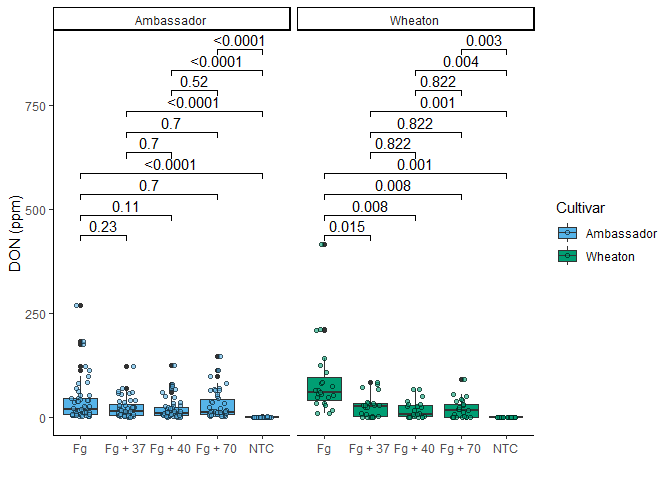
\includegraphics{Coding_challenge_markdown_files/figure-latex/P1-1.pdf}

\begin{Shaded}
\begin{Highlighting}[]
\NormalTok{P2\_stat }\OtherTok{\textless{}{-}}\NormalTok{ P2 }\SpecialCharTok{+} 
  \FunctionTok{geom\_pwc}\NormalTok{(}\FunctionTok{aes}\NormalTok{(}\AttributeTok{group =}\NormalTok{ Treatment), }\AttributeTok{method =} \StringTok{"t\_test"}\NormalTok{, }\AttributeTok{label =} \StringTok{"p.adj.format"}\NormalTok{)}
\NormalTok{P2\_stat}
\end{Highlighting}
\end{Shaded}

\begin{verbatim}
## Warning: Removed 10 rows containing non-finite outside the scale range
## (`stat_boxplot()`).
\end{verbatim}

\begin{verbatim}
## Warning: Removed 10 rows containing non-finite outside the scale range
## (`stat_pwc()`).
\end{verbatim}

\begin{verbatim}
## Warning: Removed 10 rows containing missing values or values outside the scale range
## (`geom_point()`).
\end{verbatim}

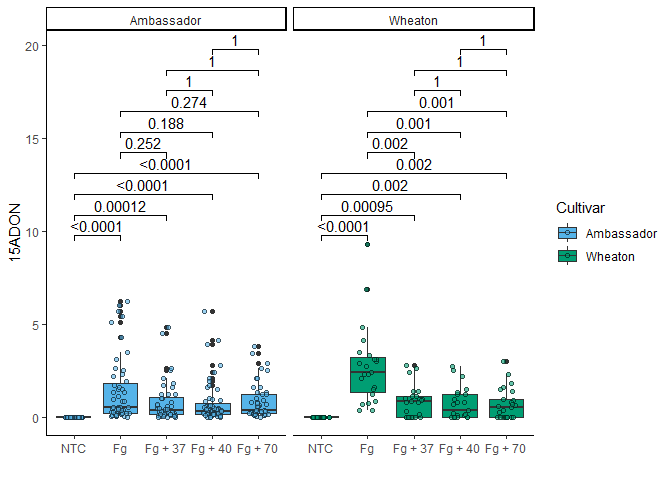
\includegraphics{Coding_challenge_markdown_files/figure-latex/P2-1.pdf}

\begin{Shaded}
\begin{Highlighting}[]
\NormalTok{P3\_stat }\OtherTok{\textless{}{-}}\NormalTok{ P3 }\SpecialCharTok{+} 
  \FunctionTok{geom\_pwc}\NormalTok{(}\FunctionTok{aes}\NormalTok{(}\AttributeTok{group =}\NormalTok{ Treatment), }\AttributeTok{method =} \StringTok{"t\_test"}\NormalTok{, }\AttributeTok{label =} \StringTok{"p.adj.format"}\NormalTok{)}
\NormalTok{P3\_stat}
\end{Highlighting}
\end{Shaded}

\begin{verbatim}
## Warning: Removed 2 rows containing non-finite outside the scale range
## (`stat_boxplot()`).
\end{verbatim}

\begin{verbatim}
## Warning: Removed 2 rows containing non-finite outside the scale range
## (`stat_pwc()`).
\end{verbatim}

\begin{verbatim}
## Warning: Removed 2 rows containing missing values or values outside the scale range
## (`geom_point()`).
\end{verbatim}

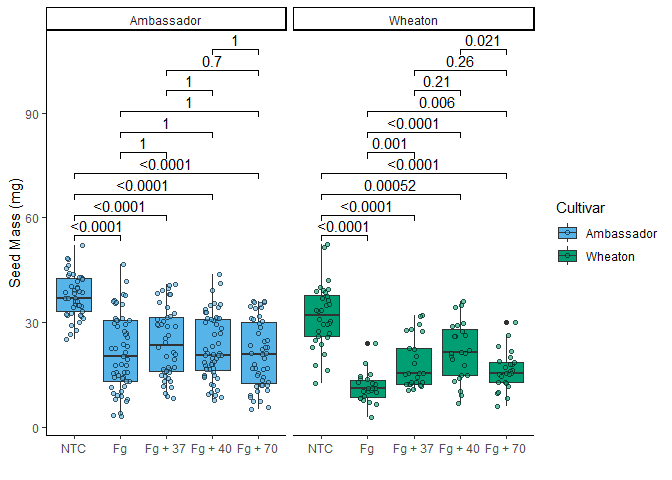
\includegraphics{Coding_challenge_markdown_files/figure-latex/P3-1.pdf}

\begin{Shaded}
\begin{Highlighting}[]
\CommentTok{\#combining}
\NormalTok{Combined\_plot\_stat }\OtherTok{\textless{}{-}} \FunctionTok{ggarrange}\NormalTok{(}
\NormalTok{  P1\_stat,   }\DocumentationTok{\#\# add the plots onf interest subsequently}
\NormalTok{  P2\_stat,}
\NormalTok{  P3\_stat,}
  \AttributeTok{labels =} \StringTok{"auto"}\NormalTok{,  }\CommentTok{\# Automatically label the plots (A, B, C, etc.)}
  \AttributeTok{nrow =} \DecValTok{1}\NormalTok{,  }\CommentTok{\# Arrange the plots in \# rows}
  \AttributeTok{ncol =} \DecValTok{3}\NormalTok{,  }\CommentTok{\# Arrange the plots in \# column}
  \AttributeTok{common.legend =}\NormalTok{ T}
\NormalTok{)}
\end{Highlighting}
\end{Shaded}

\begin{verbatim}
## Warning: Removed 8 rows containing non-finite outside the scale range
## (`stat_boxplot()`).
\end{verbatim}

\begin{verbatim}
## Warning: Removed 8 rows containing non-finite outside the scale range
## (`stat_pwc()`).
\end{verbatim}

\begin{verbatim}
## Warning: Removed 8 rows containing missing values or values outside the scale range
## (`geom_point()`).
\end{verbatim}

\begin{verbatim}
## Warning: Removed 8 rows containing non-finite outside the scale range
## (`stat_boxplot()`).
\end{verbatim}

\begin{verbatim}
## Warning: Removed 8 rows containing non-finite outside the scale range
## (`stat_pwc()`).
\end{verbatim}

\begin{verbatim}
## Warning: Removed 8 rows containing missing values or values outside the scale range
## (`geom_point()`).
\end{verbatim}

\begin{verbatim}
## Warning: Removed 10 rows containing non-finite outside the scale range
## (`stat_boxplot()`).
\end{verbatim}

\begin{verbatim}
## Warning: Removed 10 rows containing non-finite outside the scale range
## (`stat_pwc()`).
\end{verbatim}

\begin{verbatim}
## Warning: Removed 10 rows containing missing values or values outside the scale range
## (`geom_point()`).
\end{verbatim}

\begin{verbatim}
## Warning: Removed 2 rows containing non-finite outside the scale range
## (`stat_boxplot()`).
\end{verbatim}

\begin{verbatim}
## Warning: Removed 2 rows containing non-finite outside the scale range
## (`stat_pwc()`).
\end{verbatim}

\begin{verbatim}
## Warning: Removed 2 rows containing missing values or values outside the scale range
## (`geom_point()`).
\end{verbatim}

\section{Q3.Knit your document together in the following
formats:}\label{q3.knit-your-document-together-in-the-following-formats}

pdf and .md file generated by knitting

\section{Q4. 2 pts. Push the .docx or .pdf and .md files to GitHub
inside a directory called Coding Challenge
4.}\label{q4.-2-pts.-push-the-.docx-or-.pdf-and-.md-files-to-github-inside-a-directory-called-coding-challenge-4.}

bith files added to coding challenge 4 folder.
\href{https://github.com/ppg0001/PLPA_Assignment/tree/main/Coding_challenge_4}{Link}

\section{Q5. 6 pts. Now edit, commit, and push the README file for your
repository and include the following
elements.}\label{q5.-6-pts.-now-edit-commit-and-push-the-readme-file-for-your-repository-and-include-the-following-elements.}

A clickable link in your README to your GitHub flavored .md file
\href{https://github.com/ppg0001/PLPA_Assignment/blob/main/Coding_challenge_4/Coding_challenge_markdown.md}{Readme.md
Click me}

A file tree of your GitHub repository.

\begin{verbatim}
├── Coding Pracitce Assignment2_Datavis1
│   ├── Assignment_DataVis1.docx
│   ├── Assingmner_DataVis2.pdf
│   ├── Bull_richness.csv
│   └── Coding_Assignment2_DataVis.R
├── Coding Practice Assignment1_Intro
│   ├── PLPA_assignment_R1.R
│   └── TipsR.csv
├── CodingChalleng3_AdvancedVis.R
├── CodingChallenge2_IntroDataVis.R
├── Coding_Challenge1_Assignment_.R
├── Coding_challenge_4                  #ASSIGNMENT4 Main FOLDER
│   ├── Coding_challenge_markdown.md
│   └── Coding_challenge_markdown.pdf
├── Coding_challenge_markdown.html
├── Coding_challenge_markdown.md
├── Coding_challenge_markdown.pdf
├── Coding_challenge_markdown.Rmd
├── Coding_challenge_markdown_files
│   └── figure-gfm
│       ├── P1-1.png
│       ├── P2-1.png
│       └── P3-1.png
├── Coding_practice_Rmarkdown.html
├── Coding_practice_Rmarkdown.md
├── Coding_practice_Rmarkdown.Rmd
├── Coding_practice_Rmarkdown.tex
├── Coding_practice_Rmarkdown_files
│   └── figure-gfm
│       └── include the figures-1.png
├── Dummy_markdown_repo_edit_PG.Rmd
├── MycotoxinData.csv
├── PLPA_Assignment.Rproj
├── README.html
├── README.md
└── shrek.jpg
\end{verbatim}

\section{Q6. 1 pt.~Please provide me a clickable link to your
GitHub}\label{q6.-1-pt.-please-provide-me-a-clickable-link-to-your-github}

\href{https://github.com/ppg0001/PLPA_Assignment/tree/main}{Git Hub
Link}

\end{document}
